\input texbase

\titulo{Exercício Programa 23}
\materia{MAC300 - Métodos Numéricos da Álgebra Linear}

\aluno{Fernando Omar Aluani}{6797226}

\begin{document}
\cabecalho

\section{Decomposição por Valores Singulares}
A Decomposição por Valores Singulares (SVD) é um método para fatorar uma matriz A ($m\times n, m >= n$) na
forma $A = U \varSigma V^{T}$, onde:
\begin{itemize}
   \item $U$ é $m\times m$, unitária. Colunas são os vetores singulares à esquerda;
   \item $\varSigma$ é $m\times n$, diagonal. Cada elemento da diagonal é um valor singular de $A$;
   \item $V$ é $n\times n$, unitária. Colunas são os vetores singulares à direita;
\end{itemize}
Os vetores/valores singulares são relacionados aos autovetores/autovalores de uma matriz, o que faz esse método
ser muito útil para achar os autovetores e seus respectivos autovalores de uma matriz $A$.

No EP, a decomposição SVD é executada em 2 passos. O propósito do primeiro passo é "simplificar" a matriz para
a posterior diagonalização, e isso é feito com o algoritmo \textit{Golub-Kahan}. Este passo transforma a matriz
original $A$ em $A = UBV^{T}$, onde
\begin{itemize}
   \item $U$ é $m\times m$, unitária;
   \item $B$ é $m\times n$, bi-diagonal;
   \item $V$ é $n\times n$, unitária;
\end{itemize}
O segundo passo recebe $U$, $B$ e $V$, e aplicando o algoritmo \textit{Golub-Reinsch} ele diagonaliza a matriz
$B$, transformando-a na matriz $\varSigma$ e atualizando $U$ e $V$ de tal forma que $A = U \varSigma V^{T}$. 
Terminando a decomposição SVD.


\subsection{Melhorias ao método clássico}
As melhorias desse método de decomposição Golub-Kahan-Reinsch do SVD em relação ao método clássico, que usa os autovetores
e autovalores de $AA^{T}$ e $A^{T}A$, são:
\begin{itemize}
  \item É melhor para matrizes mal-condicionadas e de posto incompleto no geral;
  \item É sempre numericamente estável;
  \item É mais eficiente que a decomposição por autovalores de $AA^{T}$ ou $A^{T}A$;
\end{itemize}

\subsection{Análise da Complexidade}
Golub-Kahan é basicamente a aplicação de 2 householders ao mesmo tempo.

Golub-Reinsch vai, seguindo seu algoritmo, aplicando sucessivas rotações de Givens na matriz bidiagonal $B$, até ela
"convergir" e ser diagonalizada.

\section{Exemplo da Compressão de Imagens}
\begin{figure}[htb]
    \centering
    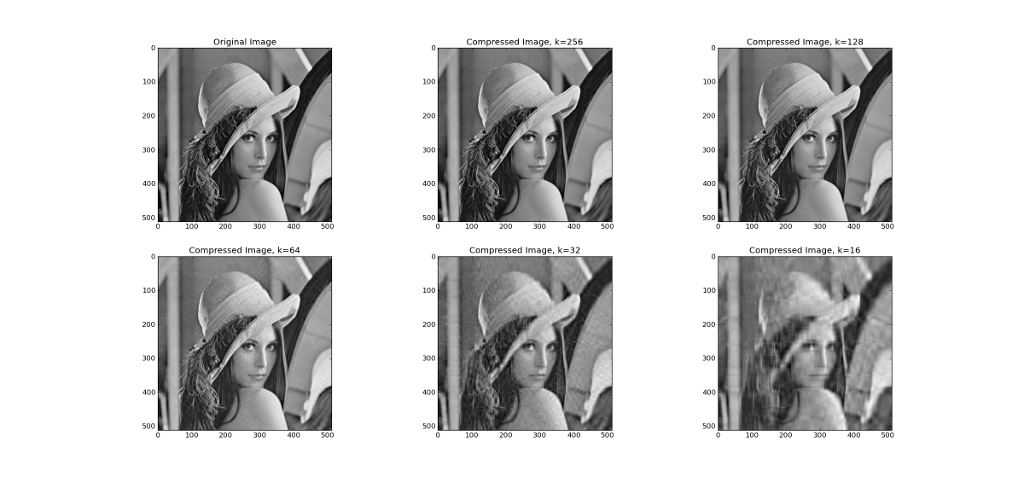
\includegraphics[width=1.0\textwidth]{grayscaleTest.png}
    \caption{Comparação de uma imagem original em grayscale e diversas compressões.}
    \label{fig:ex_gray}
\end{figure}

\begin{figure}[htb]
    \centering
    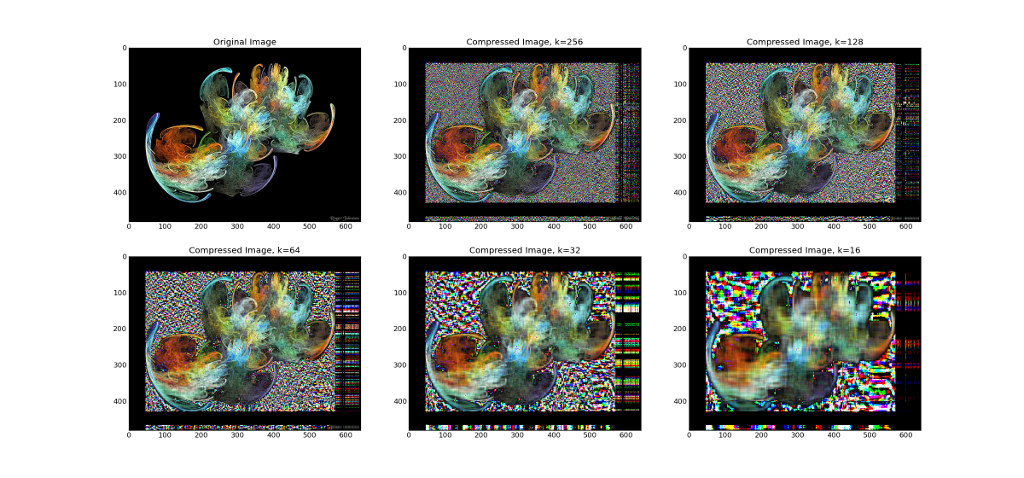
\includegraphics[width=1.0\textwidth]{rgbTest.png}
    \caption{Comparação de uma imagem original em RGB e diversas compressões. Observação: rodando o EP em si para essa 
            imagem o resultado da compressão não é o mostrado aqui. Por alguma razão que desconheço, o matplotlib desenha
            errado as imagens coloridas (nesse caso, o 'fundo' da imagem, que era preto, não passa a ser colorido de forma
            ruidosa assim)}
    \label{fig:ex_rgb}
\end{figure}


\end{document}
